\subsection{Block-based adaptive mesh refinement (AMR)}
The model geometry needs to be discretized into unique cells, in a process called meshing. For increase in accuracy, a finer mesh resolution (smaller grid size) is usually be required. Adaptive mesh refinement (AMR) takes its name from the increase in localized grid resolution to allow for improved accuracy, and this commonly results in a reduction of cost. Performing a uniform refinement over all the cells would be easier to perform, but often results in a high performance and storage cost to achieve the same effectiveness as s localized approach. Groth \etal ~\cite{Groth:1999, Williamschen:2013, Northrup:2005b, Groth:2013, zhang:2011a, zhang:2011b} developed some of the initial work with block-based AMR and extended it to enable parallel implementation for a variety of complex flows.

Block-based AMR groups cells into blocks, making it an optimal configuration for parallel systems, where each processor could have a certain number of blocks. Message Passing Interface (MPI) could be used for processor inter-communication, whereby  information exchange between the different blocks is facilitated by ghost cells that lie in the periphery of the block. Originally, the ghost cells were of the same mesh refinement level as the interior block.\par

Recently, Freret and Groth \cite{Freret:2015} have completed a new formulation for a non-uniform block-based approach that targets the the ghost cells. In this method, a block will copy over the mesh resolution and solution information of its neighboring block to its own ghost cells. This eliminates the interpolation error in multiple restriction and prolongation cycles within a uniform block-based scheme, while saving the computational cost of otherwise-necessary message passing to ensure flux conservation between the blocks. This message passing was described by Zhang~\cite{zhang:2011b} as a temporary remedy for inter-block flux evaluation applied to the ghost-cells.\par


%
\begin{figure}[t!]
\centering
    \subfigure[3D Block-Ghost configuration \cite{Rashad:2009}]
    {\label{fig:3D Block}	   
    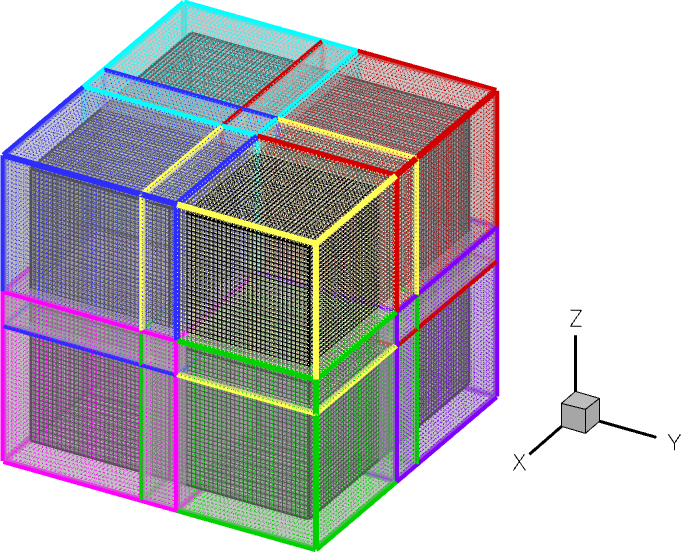
\includegraphics[height=0.35\textwidth, trim=0.2cm 0.2cm 0.2cm .2cm,clip=true]{figs/ghostblock.png}}% 
    \subfigure[Parallel domain decomposition \cite{Rashad:2009}]
    {\label{fig:3D Block}	     
    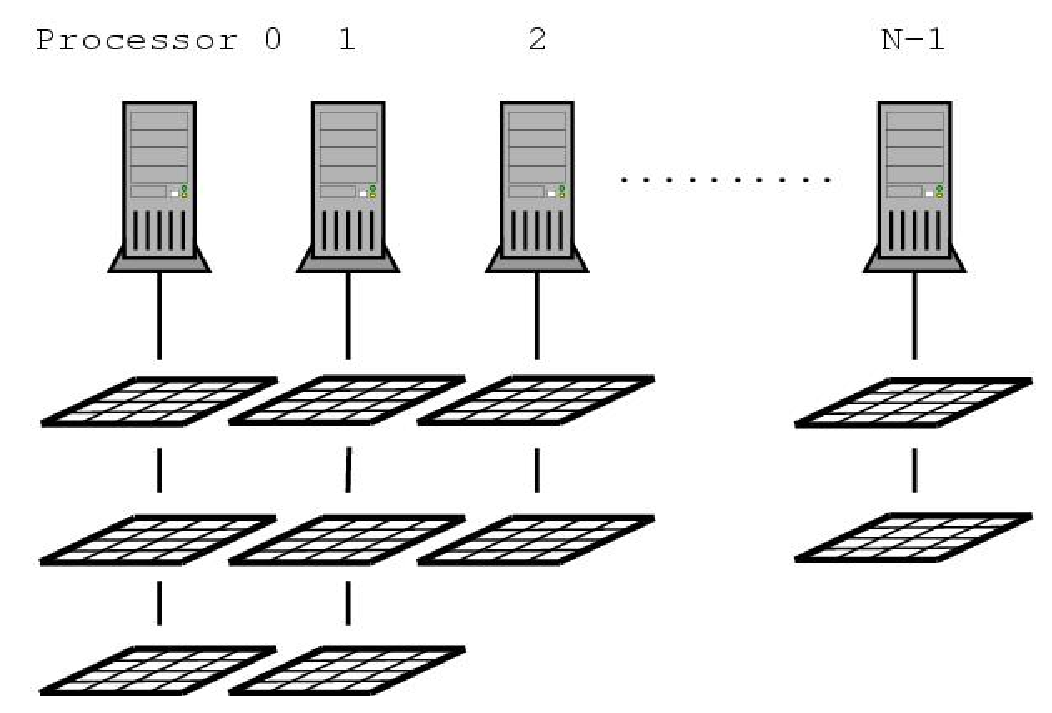
\includegraphics[height=0.35\textwidth]{./figs/parallel-domain-decomp.eps}}
\caption{The block-cell structure renders block based AMR easily parallelizable \cite{Northrup:2013}}  
\label{fig:moreAMR}
\end{figure}

Northrup and Groth~\cite{Northrup:2005b} implemented a fully-implicit, parallel Newton-Krylov method, and applies Schwarz preconditioning to take advantage of the Block structure of the computational grid.
Within block-based AMR, the cell-connectivity is stored in a tree structure, which will typically be an octree in a 3D domain. Block-Based AMR is more optimized than a refinement performed on a cell-by-cell basis, as the information storage process for the latter is computationally expensive: The tree approach is much simpler, faster and cheaper. Blocks flagged for increased resolution can be refined using two approaches: \par

%  
\begin{figure}[t!]
  \centering
   \subfigure[Isotropic and anisotropic AMR. Zhang,~\cite{zhang:2011a}]
   {\label{fig:3D Block}	   
   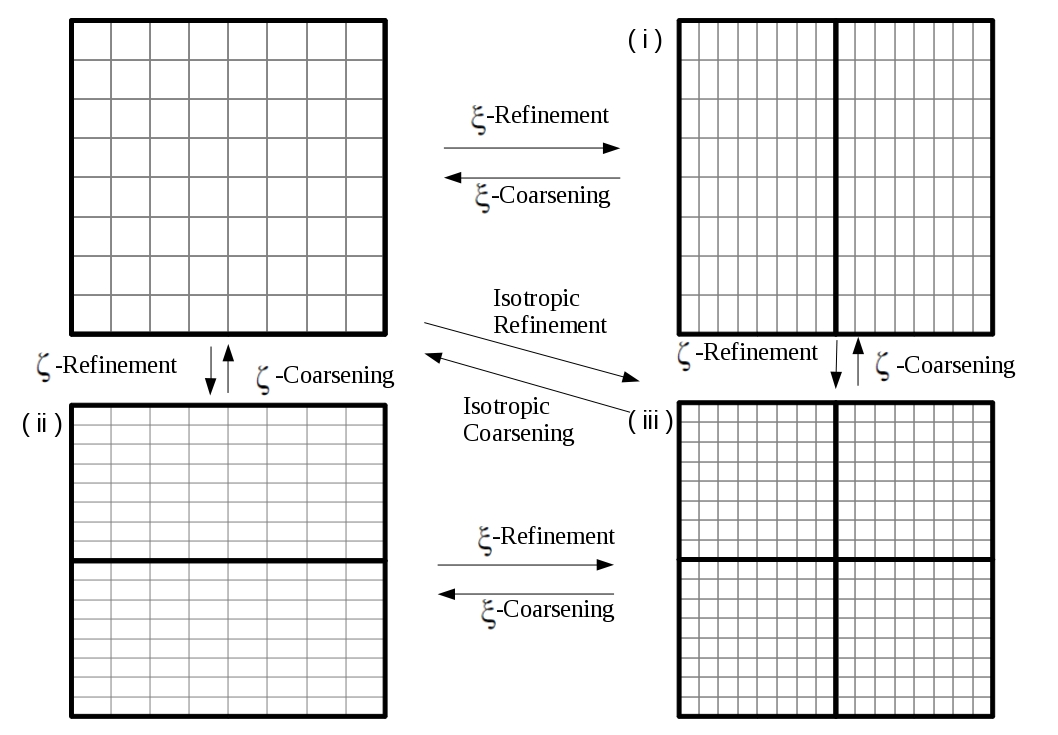
\includegraphics[height=0.35\textwidth, trim=0.2cm 0.2cm 0.2cm .2cm,clip=true]{figs/BlockDivision.jpg}}%
   \subfigure[Non-uniform block structure, Freret and Groth~\cite{Freret:2015}]
   {\label{fig:nonUni}	   
   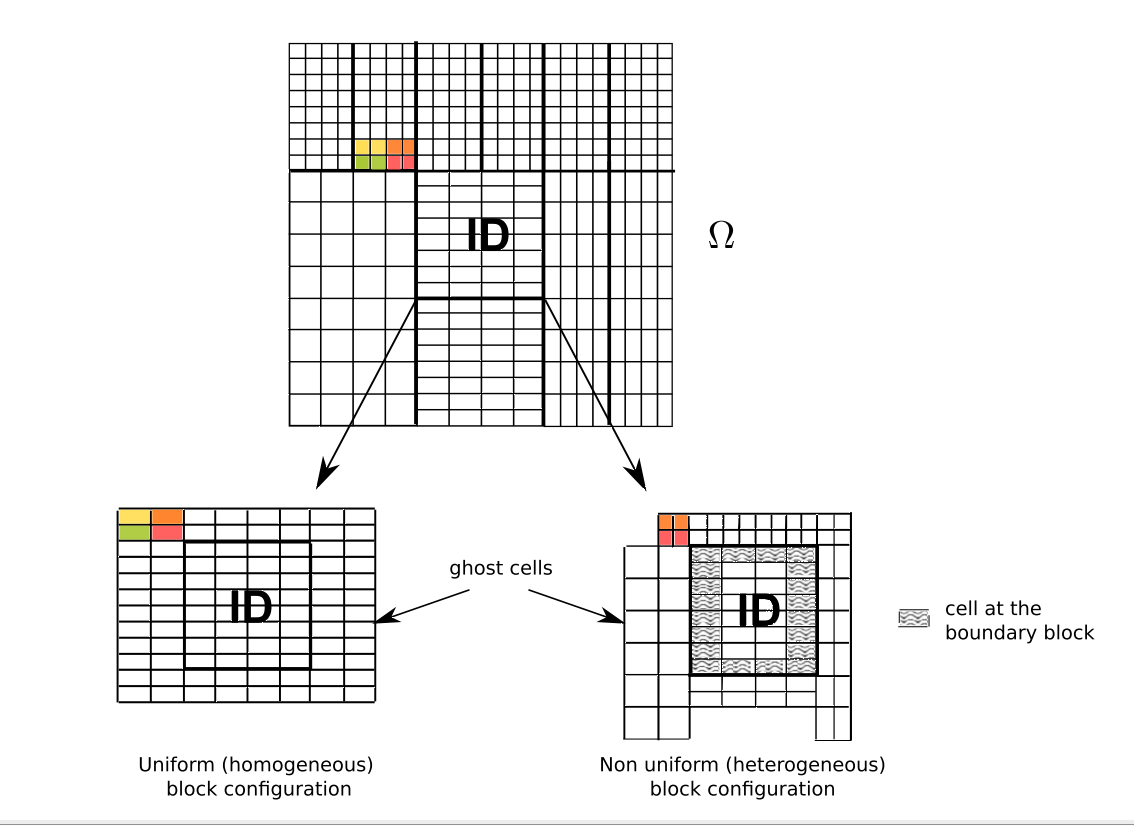
\includegraphics[height=0.42\textwidth, trim=2cm 0cm 9cm 0cm,clip=true]{./figs/Non-UniformBlock.png}}%  
\caption{Block structure depicting interior cells and ghost cell configurations} 
\label{fig:unifNon}    
\end{figure}  
  

\begin{enumerate}

\item \textbf{Isotropic AMR}:\\
Isotropic AMR  occurs by uniformly splitting the Parent cell into 8 children (in a 3D domain) or into 4 children (in a 2D domain). This considers that the physics is occurring without a preference for a given direction, and usually results in a larger-than-desired cell count.


\item \textbf{Anisotropic AMR}: \\
For flows with directional bulk bias it can be predicted that mesh cells would ideally be stretched along this axis. Anisotropy refers to a preference in mesh refinement axes. Studies by Zhang ~\cite{zhang:2011a}, Zhang and Groth ~\cite{zhang:2011b}, Freret and Groth ~\cite{Freret:2015} indicate that anisotropic AMR for given simulations result in lower cell counts (see figure \ref{fig:isoAniso}), although the refinement procedure is more difficult than that of the Isotropic AMR. \par

\end{enumerate}

\begin{figure}[t!]
  \centering
	\subfigure[Initial density (t=0s) obtained after 6 initial  refinements. 14057 blocks]
   {\label{fig:iso0}	   
   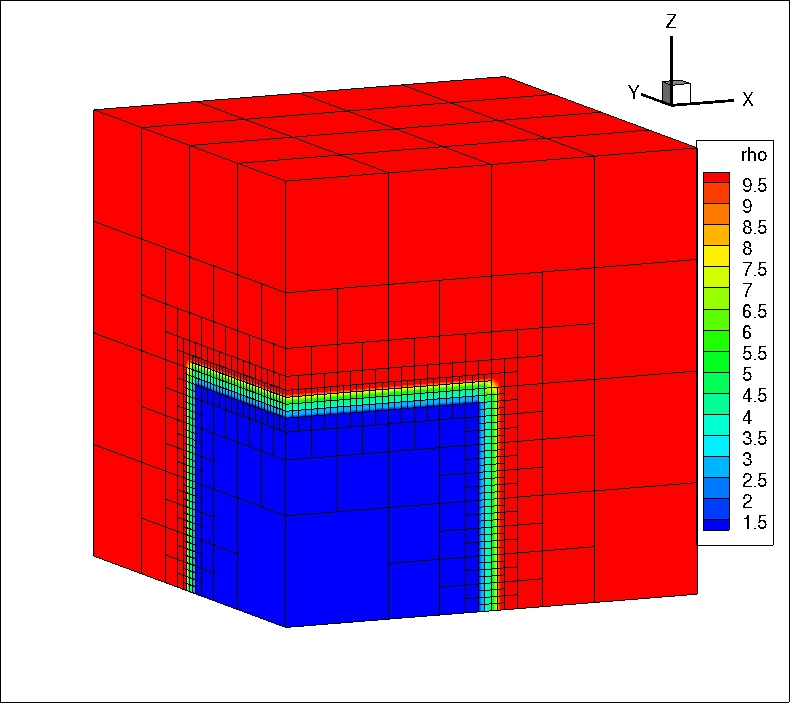
\includegraphics[height=0.2\textwidth]{figs/shockCubeIso0.jpg}}%
   \:
   \subfigure[Density (at t=0.5s). 7036 blocks.]
   {\label{fig:iso3}	   
   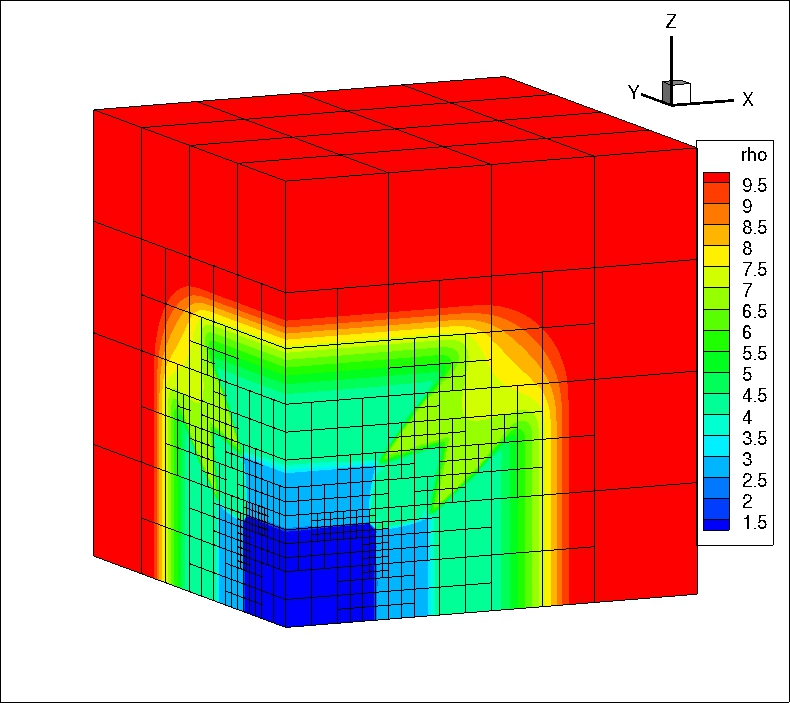
\includegraphics[height=0.2\textwidth]{figs/shockCubeIso3.jpg}}%
	\:
	\subfigure[Initial density (t=0s) obtained after 6 initial refinements. 1089 blocks. ]
   {\label{fig:Aniso0}	   
   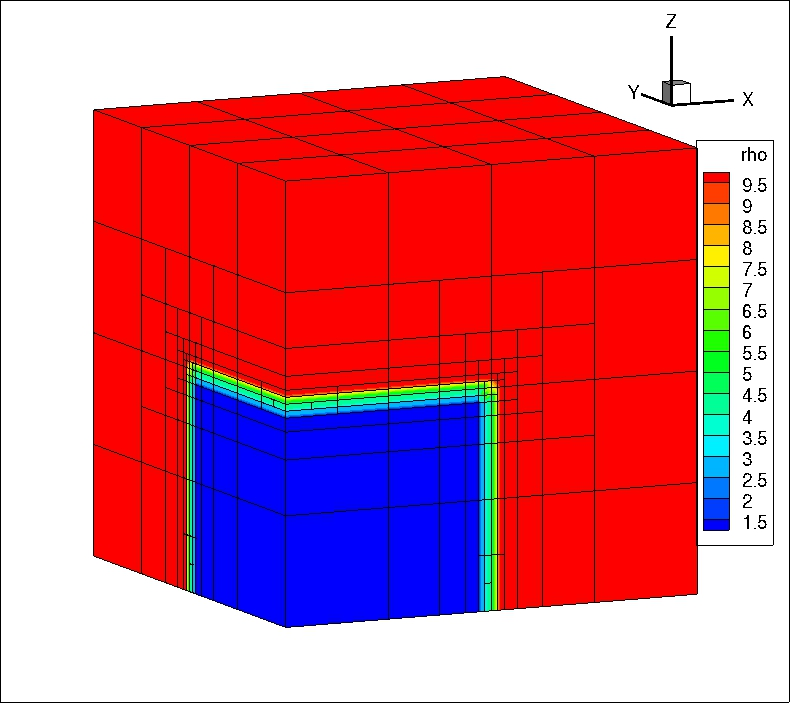
\includegraphics[height=0.2\textwidth]{figs/shockCubeAniso0.jpg}}%
   \:
	\subfigure[Density (at t=0.5s). 5522 blocks]
   {\label{fig:Aniso3}	   
   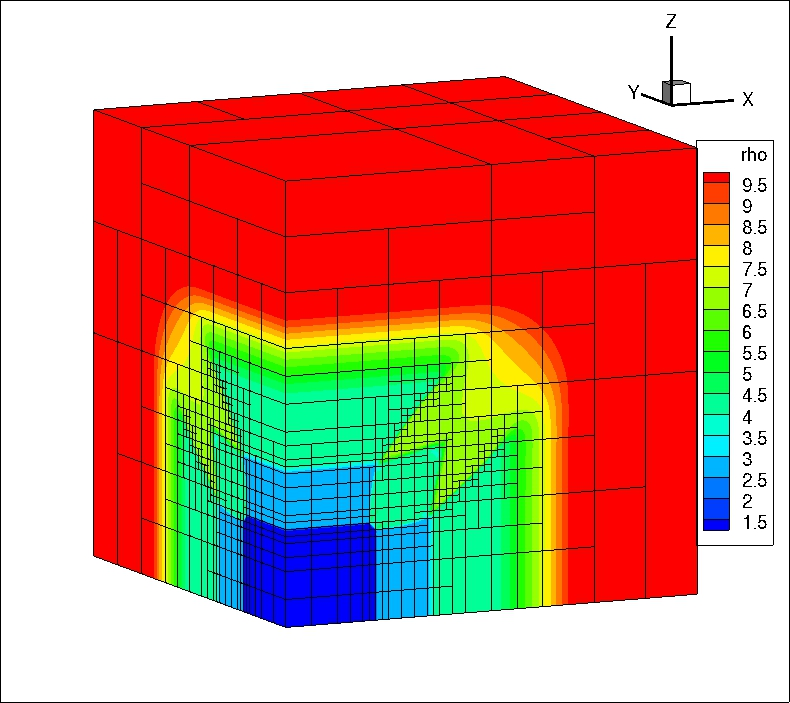
\includegraphics[height=0.2\textwidth]{figs/shockCubeAniso3.jpg}}%
   \caption{Differences between the isotropic and anisotropic AMR on a shockcube problem. Initial conditions have large density jumps between left and right states: 1 block = 8x8x8 cells. For this case, a savings of $\approx 28\%$ in cell count is achieved by the anisotropic method. [Freret and Groth: 2015] \cite{Freret:2015} } 
\label{fig:isoAniso}      
\end{figure}  



